To quantify the effectiveness of this method we compare it to the existing OpenDataCam tool.
We will compare the counts, produced by OpenDataCam and manual annotation, of cyclists at strategic parts of the intersection with the counts produced by our system. The manually annotated counts being the ground truth.
This is followed by an analysis of the desire paths and an analysis of body language when cyclist trigger a defined
alert zone.
\ \\ 

\subsubsection{Comparison between three different methods}
Table x shows a comparison between OpenDataCam, manual annotation and our method.
The comparison is based on how well each method captured cyclists driving on along three different 
desire lines towards Fisketorvet.
Our method captured x ‰ of what manual annotation has, manual annotation being the baseline.
\ \\

\subsubsection{Interpretation of desire paths desire paths}
The trajectory analysis in Figure~\ref{Rainbow} we can determine eight commonly taken desire paths. 
Whereas with manual annotation we can determine x amount.
\ \\
\raggedbottom
\ \\ 
\noindent
\begin{tabular}{@{}cc}
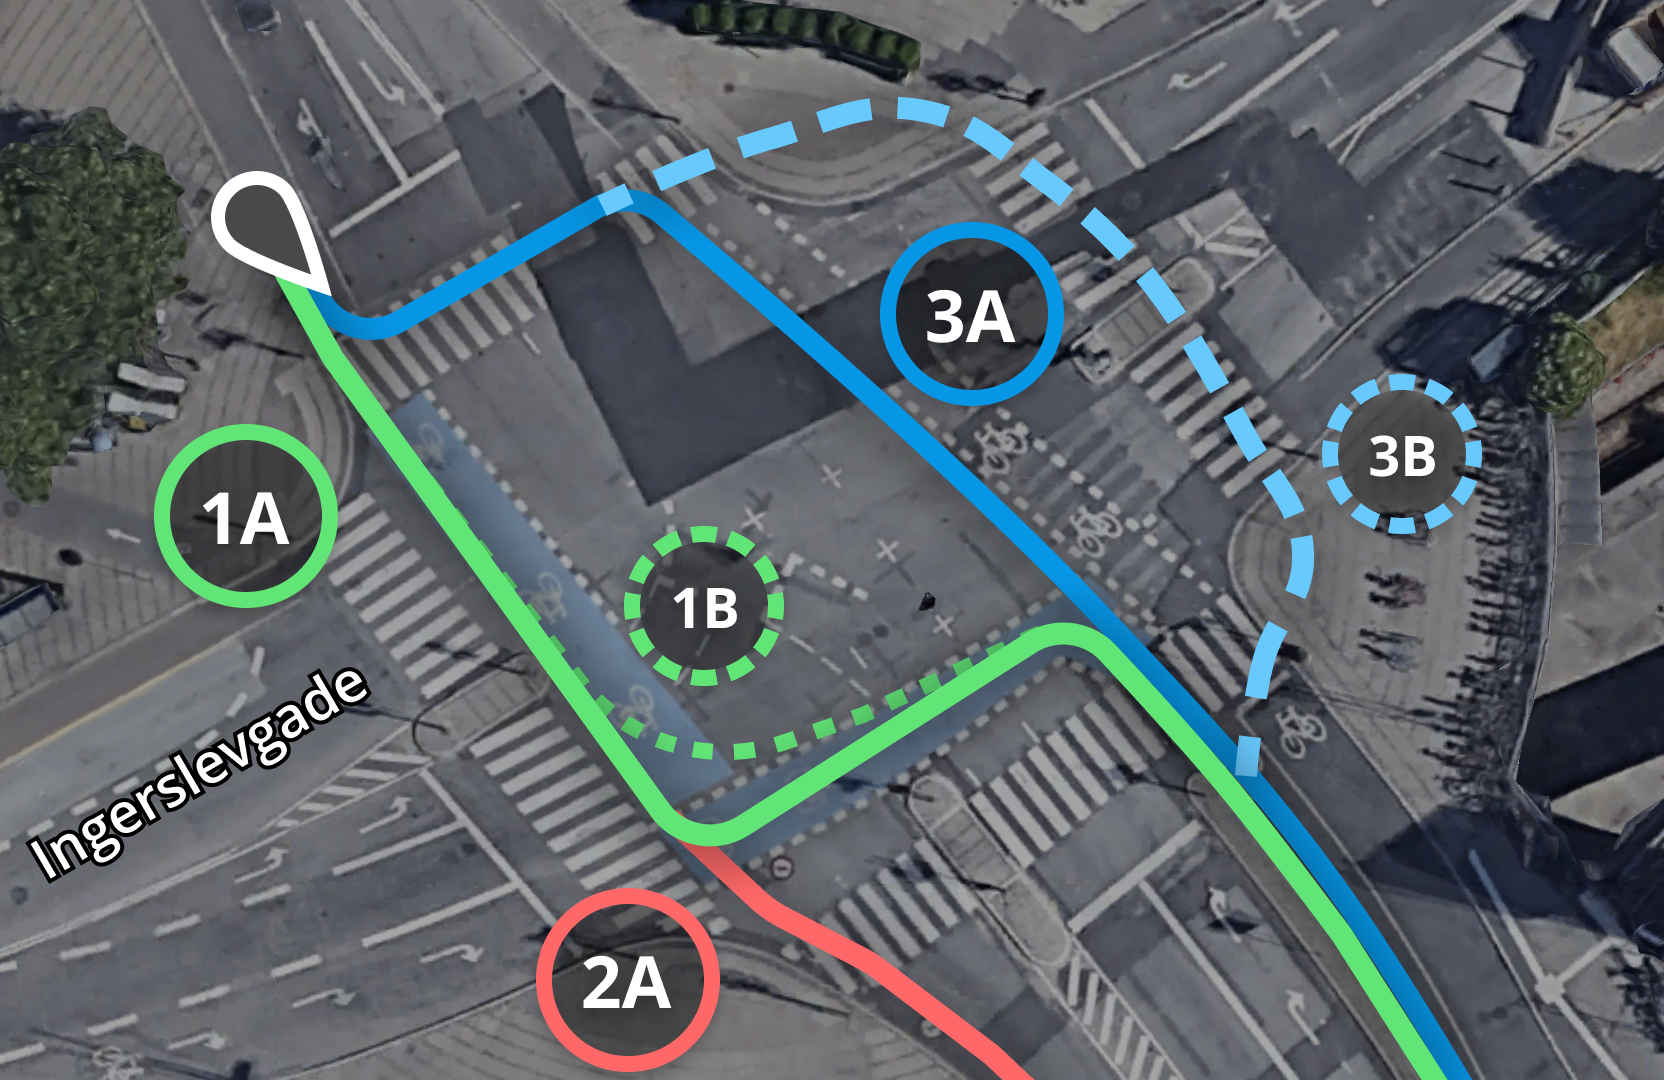
\includegraphics[width=1.0\columnwidth]{desire_paths_overhead} 
\end{tabular}
\captionof{figure}{Common trajectories of cyclists coming from NW}
\label{traject}

\ \\
\subsubsection{behavioral analysis}
As mentioned in the web application, we couple the top-level view with references to timestamps in the recorded footage, 
such that the behavior of cyclists can be observed at street level.
Whenever a unique trajectory is selected or a part of the intersection is marked off, one can inspect each individual cyclist 
and the context leading up to a detection.
\\

In the below image we see a typical detection of a rider passing straight over Dybbølsbro instead of turning left and 
continuing over the bi-directional cycle path. Unknowingly thinking he is in the right, he closely passes, at full speed, another rider crossing
the street. Shortly after he notices the traffic markings and turns around. 

\ \\ 
\raggedbottom
\begin{tabular}{@{}cc}
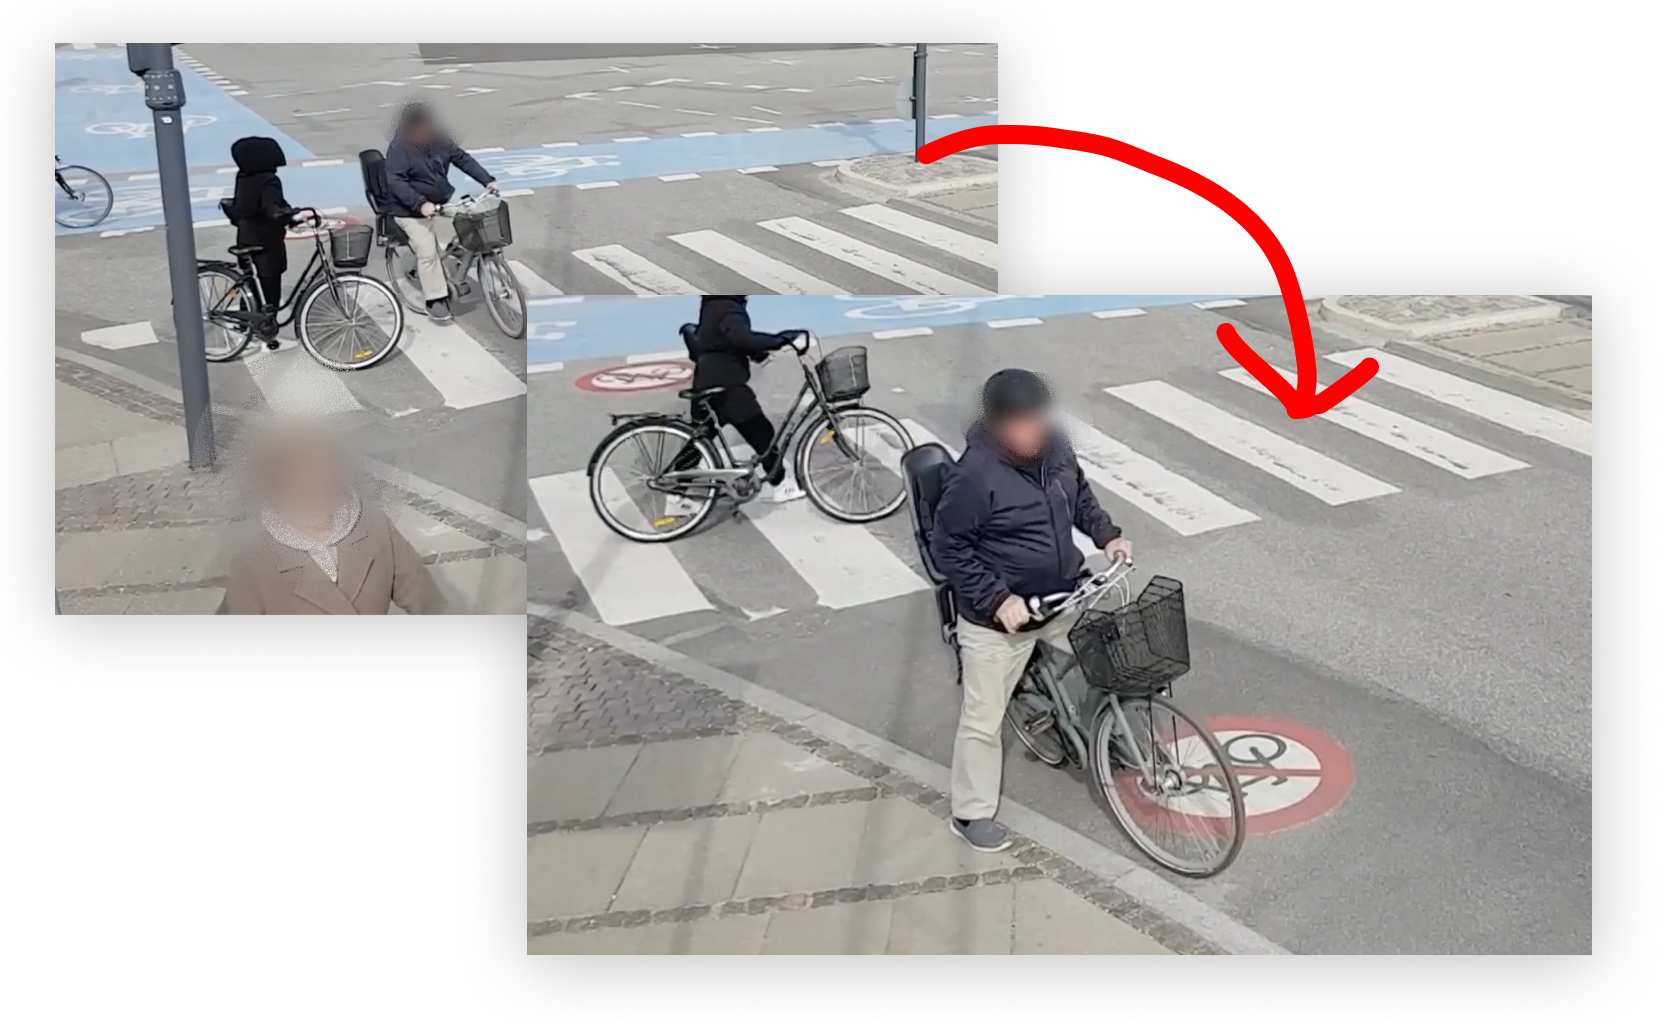
\includegraphics[width=1.0\columnwidth]{behaviour_fast} 
\end{tabular}
\captionof{figure}{Detection zone triggered}
\label{Alert}
\ \\

Another commonly observed behavior was cyclists trying to shorten the trajectories of their turns 
at the "waiting corner" at Ingerslevgade.

\raggedbottom
\ \\ 
\noindent
\begin{tabular}{@{}cc}
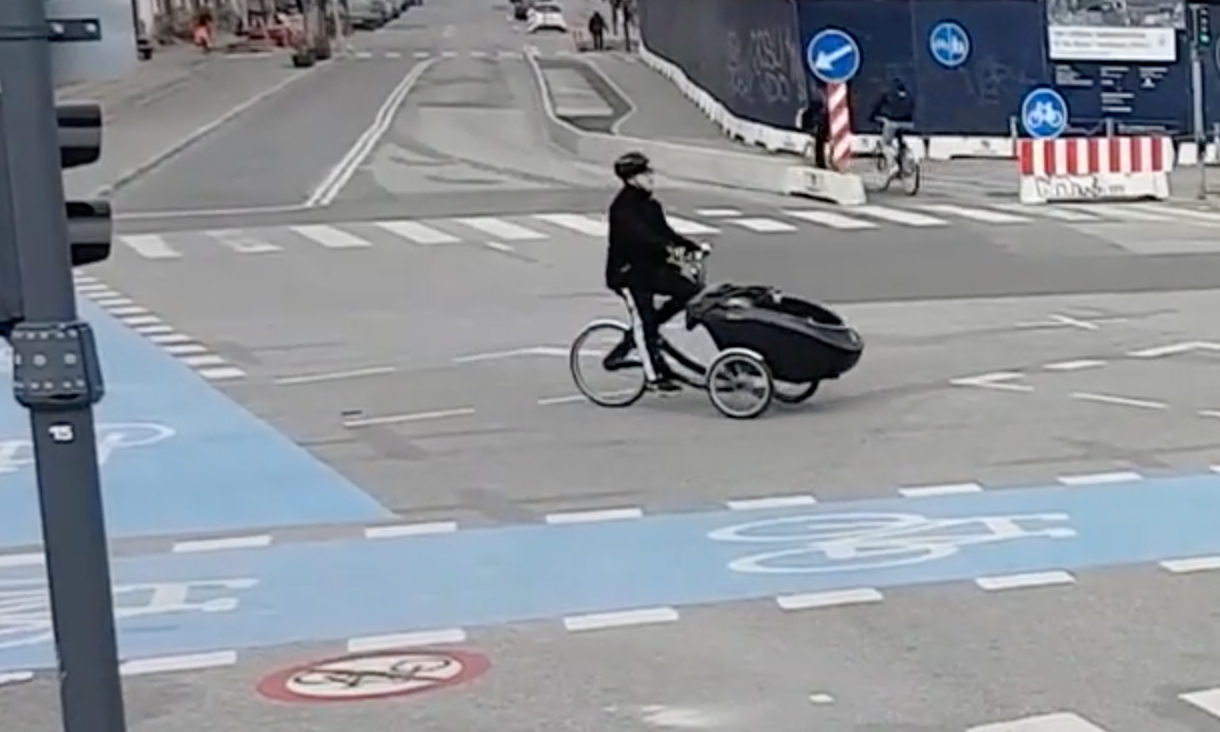
\includegraphics[width=1.0\columnwidth]{shorten_traj} 
\end{tabular}
\captionof{figure}{Shortend turn}
\label{Alert}
\ \\

When volumes of other traffic were low or over the short window of all traffic having red lights, cyclists would use the opportunity 
to swiftly cross the intersection while still "following the correct path" (that is, not crossing in a fully diagonal path). 

% Which are all compared to the "ground truth" dataset that we annotate manually. We know from previous works with OpenDataCam
% that vehicle detection has achieved 95\% accuracy while performing worse for pedestrians and motorcycles (\cite{BROEKMAN2021100068}).

